\documentclass[1p]{elsarticle_modified}
%\bibliographystyle{elsarticle-num}

%\usepackage[colorlinks]{hyperref}
%\usepackage{abbrmath_seonhwa} %\Abb, \Ascr, \Acal ,\Abf, \Afrak
\usepackage{amsfonts}
\usepackage{amssymb}
\usepackage{amsmath}
\usepackage{amsthm}
\usepackage{scalefnt}
\usepackage{amsbsy}
\usepackage{kotex}
\usepackage{caption}
\usepackage{subfig}
\usepackage{color}
\usepackage{graphicx}
\usepackage{xcolor} %% white, black, red, green, blue, cyan, magenta, yellow
\usepackage{float}
\usepackage{setspace}
\usepackage{hyperref}

\usepackage{tikz}
\usetikzlibrary{arrows}

\usepackage{multirow}
\usepackage{array} % fixed length table
\usepackage{hhline}

%%%%%%%%%%%%%%%%%%%%%
\makeatletter
\renewcommand*\env@matrix[1][\arraystretch]{%
	\edef\arraystretch{#1}%
	\hskip -\arraycolsep
	\let\@ifnextchar\new@ifnextchar
	\array{*\c@MaxMatrixCols c}}
\makeatother %https://tex.stackexchange.com/questions/14071/how-can-i-increase-the-line-spacing-in-a-matrix
%%%%%%%%%%%%%%%

\usepackage[normalem]{ulem}

\newcommand{\msout}[1]{\ifmmode\text{\sout{\ensuremath{#1}}}\else\sout{#1}\fi}
%SOURCE: \msout is \stkout macro in https://tex.stackexchange.com/questions/20609/strikeout-in-math-mode

\newcommand{\cancel}[1]{
	\ifmmode
	{\color{red}\msout{#1}}
	\else
	{\color{red}\sout{#1}}
	\fi
}

\newcommand{\add}[1]{
	{\color{blue}\uwave{#1}}
}

\newcommand{\replace}[2]{
	\ifmmode
	{\color{red}\msout{#1}}{\color{blue}\uwave{#2}}
	\else
	{\color{red}\sout{#1}}{\color{blue}\uwave{#2}}
	\fi
}

\newcommand{\Sol}{\mathcal{S}} %segment
\newcommand{\D}{D} %diagram
\newcommand{\A}{\mathcal{A}} %arc


%%%%%%%%%%%%%%%%%%%%%%%%%%%%%5 test

\def\sl{\operatorname{\textup{SL}}(2,\Cbb)}
\def\psl{\operatorname{\textup{PSL}}(2,\Cbb)}
\def\quan{\mkern 1mu \triangleright \mkern 1mu}

\theoremstyle{definition}
\newtheorem{thm}{Theorem}[section]
\newtheorem{prop}[thm]{Proposition}
\newtheorem{lem}[thm]{Lemma}
\newtheorem{ques}[thm]{Question}
\newtheorem{cor}[thm]{Corollary}
\newtheorem{defn}[thm]{Definition}
\newtheorem{exam}[thm]{Example}
\newtheorem{rmk}[thm]{Remark}
\newtheorem{alg}[thm]{Algorithm}

\newcommand{\I}{\sqrt{-1}}
\begin{document}

%\begin{frontmatter}
%
%\title{Boundary parabolic representations of knots up to 8 crossings}
%
%%% Group authors per affiliation:
%\author{Yunhi Cho} 
%\address{Department of Mathematics, University of Seoul, Seoul, Korea}
%\ead{yhcho@uos.ac.kr}
%
%
%\author{Seonhwa Kim} %\fnref{s_kim}}
%\address{Center for Geometry and Physics, Institute for Basic Science, Pohang, 37673, Korea}
%\ead{ryeona17@ibs.re.kr}
%
%\author{Hyuk Kim}
%\address{Department of Mathematical Sciences, Seoul National University, Seoul 08826, Korea}
%\ead{hyukkim@snu.ac.kr}
%
%\author{Seokbeom Yoon}
%\address{Department of Mathematical Sciences, Seoul National University, Seoul, 08826,  Korea}
%\ead{sbyoon15@snu.ac.kr}
%
%\begin{abstract}
%We find all boundary parabolic representation of knots up to 8 crossings.
%
%\end{abstract}
%\begin{keyword}
%    \MSC[2010] 57M25 
%\end{keyword}
%
%\end{frontmatter}

%\linenumbers
%\tableofcontents
%
\newcommand\colored[1]{\textcolor{white}{\rule[-0.35ex]{0.8em}{1.4ex}}\kern-0.8em\color{red} #1}%
%\newcommand\colored[1]{\textcolor{white}{ #1}\kern-2.17ex	\textcolor{white}{ #1}\kern-1.81ex	\textcolor{white}{ #1}\kern-2.15ex\color{red}#1	}

{\Large $\underline{12a_{0334}~(K12a_{0334})}$}

\setlength{\tabcolsep}{10pt}
\renewcommand{\arraystretch}{1.6}
\vspace{1cm}\begin{tabular}{m{100pt}>{\centering\arraybackslash}m{274pt}}
\multirow{5}{120pt}{
	\centering
	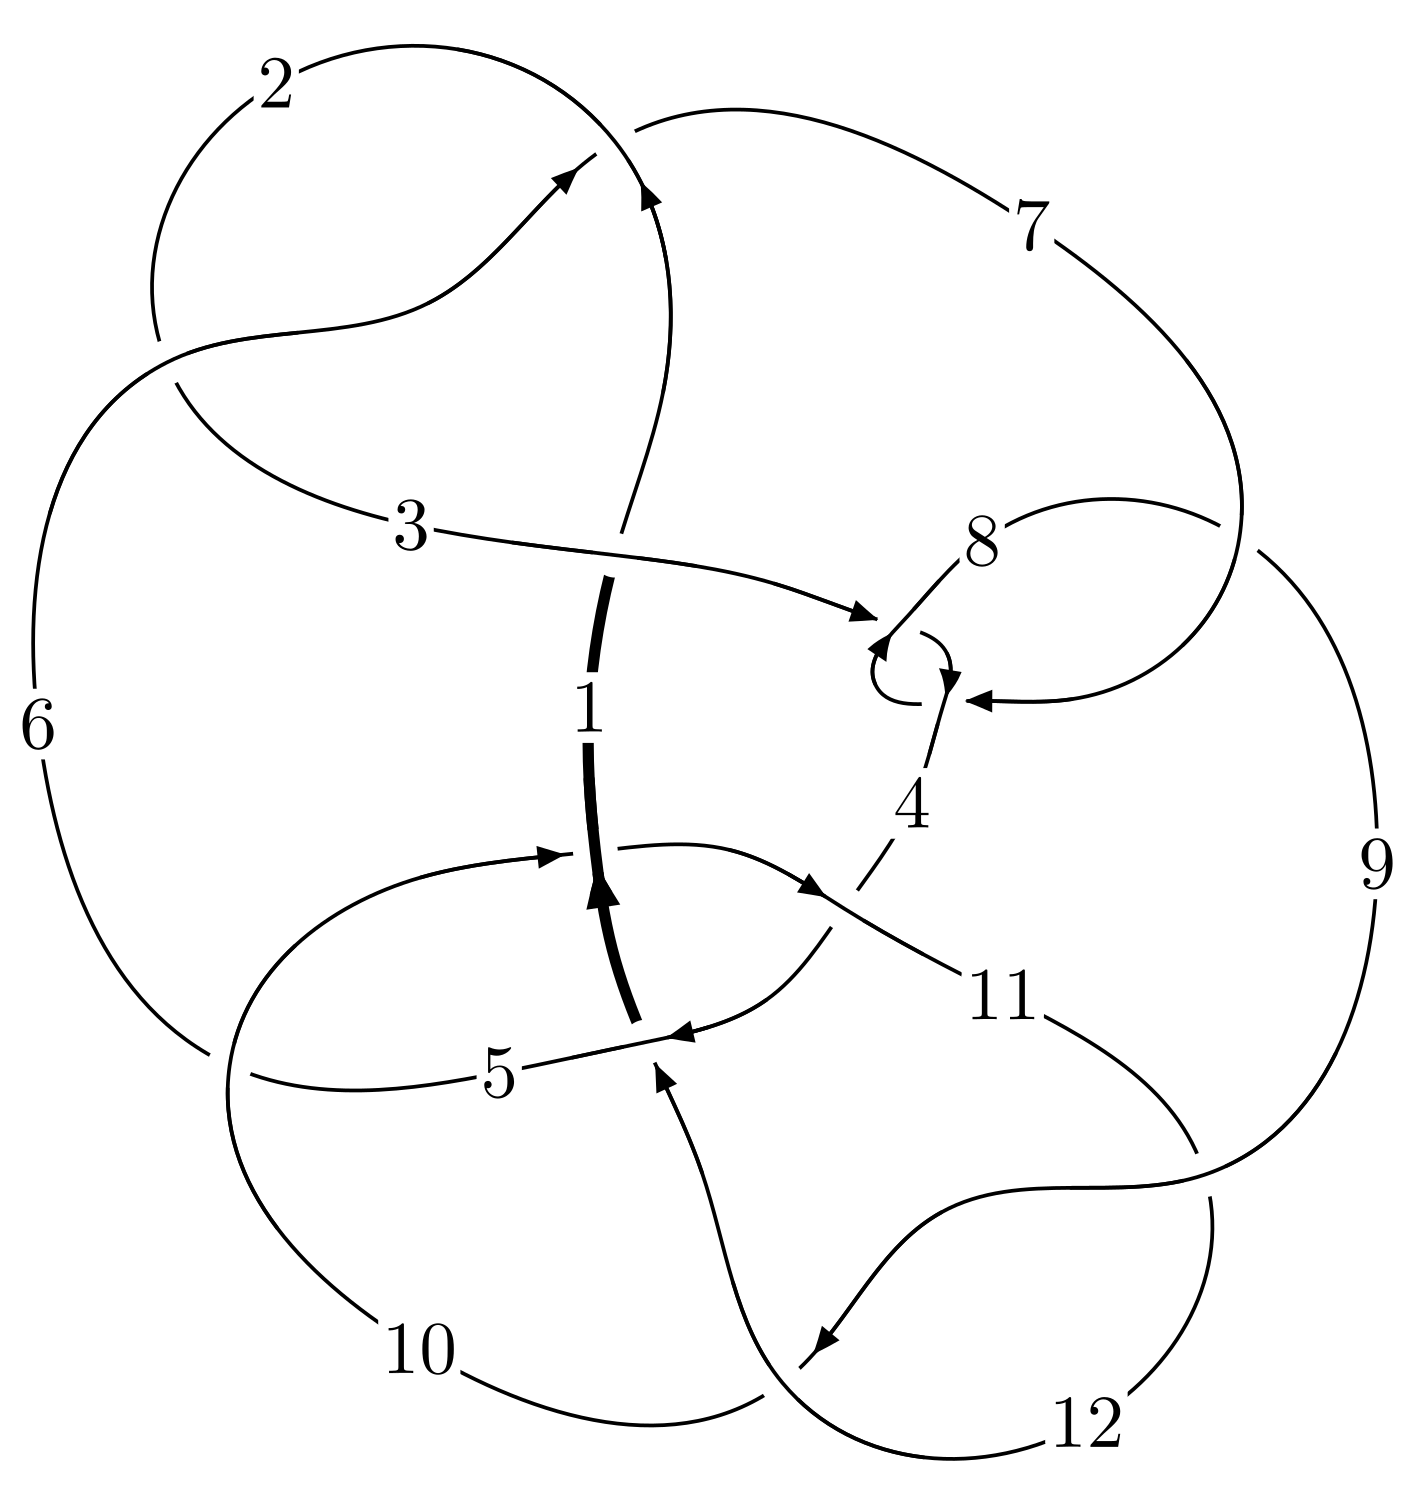
\includegraphics[width=112pt]{../../../GIT/diagram.site/Diagrams/png/1135_12a_0334.png}\\
\ \ \ A knot diagram\footnotemark}&
\allowdisplaybreaks
\textbf{Linearized knot diagam} \\
\cline{2-2}
 &
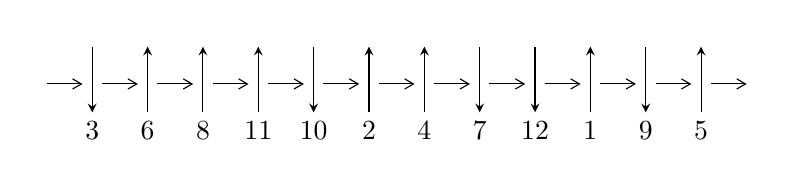
\begin{tikzpicture}[x=20pt, y=17pt]
	% nodes
	\node (C0) at (0, 0) {};
	\node (C1) at (1, 0) {};
	\node (C1U) at (1, +1) {};
	\node (C1D) at (1, -1) {3};

	\node (C2) at (2, 0) {};
	\node (C2U) at (2, +1) {};
	\node (C2D) at (2, -1) {6};

	\node (C3) at (3, 0) {};
	\node (C3U) at (3, +1) {};
	\node (C3D) at (3, -1) {8};

	\node (C4) at (4, 0) {};
	\node (C4U) at (4, +1) {};
	\node (C4D) at (4, -1) {11};

	\node (C5) at (5, 0) {};
	\node (C5U) at (5, +1) {};
	\node (C5D) at (5, -1) {10};

	\node (C6) at (6, 0) {};
	\node (C6U) at (6, +1) {};
	\node (C6D) at (6, -1) {2};

	\node (C7) at (7, 0) {};
	\node (C7U) at (7, +1) {};
	\node (C7D) at (7, -1) {4};

	\node (C8) at (8, 0) {};
	\node (C8U) at (8, +1) {};
	\node (C8D) at (8, -1) {7};

	\node (C9) at (9, 0) {};
	\node (C9U) at (9, +1) {};
	\node (C9D) at (9, -1) {12};

	\node (C10) at (10, 0) {};
	\node (C10U) at (10, +1) {};
	\node (C10D) at (10, -1) {1};

	\node (C11) at (11, 0) {};
	\node (C11U) at (11, +1) {};
	\node (C11D) at (11, -1) {9};

	\node (C12) at (12, 0) {};
	\node (C12U) at (12, +1) {};
	\node (C12D) at (12, -1) {5};
	\node (C13) at (13, 0) {};

	% arrows
	\draw[->,>={angle 60}]
	(C0) edge (C1) (C1) edge (C2) (C2) edge (C3) (C3) edge (C4) (C4) edge (C5) (C5) edge (C6) (C6) edge (C7) (C7) edge (C8) (C8) edge (C9) (C9) edge (C10) (C10) edge (C11) (C11) edge (C12) (C12) edge (C13) ;	\draw[->,>=stealth]
	(C1U) edge (C1D) (C2D) edge (C2U) (C3D) edge (C3U) (C4D) edge (C4U) (C5U) edge (C5D) (C6D) edge (C6U) (C7D) edge (C7U) (C8U) edge (C8D) (C9U) edge (C9D) (C10D) edge (C10U) (C11U) edge (C11D) (C12D) edge (C12U) ;
	\end{tikzpicture} \\
\hhline{~~} \\& 
\textbf{Solving Sequence} \\ \cline{2-2} 
 &
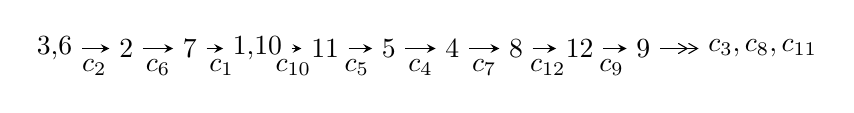
\begin{tikzpicture}[x=23pt, y=7pt]
	% node
	\node (A0) at (-1/8, 0) {3,6};
	\node (A1) at (1, 0) {2};
	\node (A2) at (2, 0) {7};
	\node (A3) at (49/16, 0) {1,10};
	\node (A4) at (33/8, 0) {11};
	\node (A5) at (41/8, 0) {5};
	\node (A6) at (49/8, 0) {4};
	\node (A7) at (57/8, 0) {8};
	\node (A8) at (65/8, 0) {12};
	\node (A9) at (73/8, 0) {9};
	\node (C1) at (1/2, -1) {$c_{2}$};
	\node (C2) at (3/2, -1) {$c_{6}$};
	\node (C3) at (5/2, -1) {$c_{1}$};
	\node (C4) at (29/8, -1) {$c_{10}$};
	\node (C5) at (37/8, -1) {$c_{5}$};
	\node (C6) at (45/8, -1) {$c_{4}$};
	\node (C7) at (53/8, -1) {$c_{7}$};
	\node (C8) at (61/8, -1) {$c_{12}$};
	\node (C9) at (69/8, -1) {$c_{9}$};
	\node (A10) at (11, 0) {$c_{3},c_{8},c_{11}$};

	% edge
	\draw[->,>=stealth]	
	(A0) edge (A1) (A1) edge (A2) (A2) edge (A3) (A3) edge (A4) (A4) edge (A5) (A5) edge (A6) (A6) edge (A7) (A7) edge (A8) (A8) edge (A9) ;
	\draw[->>,>={angle 60}]	
	(A9) edge (A10);
\end{tikzpicture} \\ 

\end{tabular} \\

\footnotetext{
The image of knot diagram is generated by the software ``\textbf{Draw programme}" developed by Andrew Bartholomew(\url{http://www.layer8.co.uk/maths/draw/index.htm\#Running-draw}), where we modified some parts for our purpose(\url{https://github.com/CATsTAILs/LinksPainter}).
}\phantom \\ \newline 
\centering \textbf{Ideals for irreducible components\footnotemark of $X_{\text{par}}$} 
 
\begin{align*}
I^u_{1}&=\langle 
2.06298\times10^{20} u^{52}+1.60476\times10^{20} u^{51}+\cdots+4.29074\times10^{20} b-4.12339\times10^{20},\\
\phantom{I^u_{1}}&\phantom{= \langle  }1.99532\times10^{20} u^{52}+2.05042\times10^{20} u^{51}+\cdots+2.14537\times10^{20} a-6.01161\times10^{20},\;u^{53}+u^{52}+\cdots- u+1\rangle \\
I^u_{2}&=\langle 
8.20708\times10^{90} u^{81}+1.10415\times10^{91} u^{80}+\cdots+2.42746\times10^{91} b+4.21770\times10^{91},\\
\phantom{I^u_{2}}&\phantom{= \langle  }-1.38634\times10^{91} u^{81}+4.31343\times10^{91} u^{80}+\cdots+4.12668\times10^{92} a+3.38112\times10^{93},\\
\phantom{I^u_{2}}&\phantom{= \langle  }u^{82}+u^{81}+\cdots+80 u+17\rangle \\
I^u_{3}&=\langle 
a^4- a^3 u+2 a^2- a u+b- a+u+2,\;a^5+a^4+2 a^3+a^2+a+1,\;u^2+1\rangle \\
I^u_{4}&=\langle 
4 b-1,\;2 a-1,\;u+1\rangle \\
\\
\end{align*}
\raggedright * 4 irreducible components of $\dim_{\mathbb{C}}=0$, with total 146 representations.\\
\footnotetext{All coefficients of polynomials are rational numbers. But the coefficients are sometimes approximated in decimal forms when there is not enough margin.}
\newpage
\renewcommand{\arraystretch}{1}
\centering \section*{I. $I^u_{1}= \langle 2.06\times10^{20} u^{52}+1.60\times10^{20} u^{51}+\cdots+4.29\times10^{20} b-4.12\times10^{20},\;2.00\times10^{20} u^{52}+2.05\times10^{20} u^{51}+\cdots+2.15\times10^{20} a-6.01\times10^{20},\;u^{53}+u^{52}+\cdots- u+1 \rangle$}
\flushleft \textbf{(i) Arc colorings}\\
\begin{tabular}{m{7pt} m{180pt} m{7pt} m{180pt} }
\flushright $a_{3}=$&$\begin{pmatrix}1\\0\end{pmatrix}$ \\
\flushright $a_{6}=$&$\begin{pmatrix}0\\u\end{pmatrix}$ \\
\flushright $a_{2}=$&$\begin{pmatrix}1\\u^2\end{pmatrix}$ \\
\flushright $a_{7}=$&$\begin{pmatrix}u\\u^3+u\end{pmatrix}$ \\
\flushright $a_{1}=$&$\begin{pmatrix}u^2+1\\u^2\end{pmatrix}$ \\
\flushright $a_{10}=$&$\begin{pmatrix}-0.930057 u^{52}-0.955742 u^{51}+\cdots-6.21940 u+2.80213\\-0.480798 u^{52}-0.374006 u^{51}+\cdots-2.83945 u+0.960996\end{pmatrix}$ \\
\flushright $a_{11}=$&$\begin{pmatrix}-1.04871 u^{52}-0.780472 u^{51}+\cdots-8.33773 u+3.26868\\0.0764895 u^{52}+0.115237 u^{51}+\cdots-1.80155 u+0.599031\end{pmatrix}$ \\
\flushright $a_{5}=$&$\begin{pmatrix}0.000620096 u^{52}+0.181918 u^{51}+\cdots-5.81545 u+4.31836\\-0.579013 u^{52}-0.551580 u^{51}+\cdots-2.53269 u+0.624293\end{pmatrix}$ \\
\flushright $a_{4}=$&$\begin{pmatrix}-0.0312500 u^{51}-0.0312500 u^{50}+\cdots+0.0312500 u+0.968750\\- u^2\end{pmatrix}$ \\
\flushright $a_{8}=$&$\begin{pmatrix}-0.0312500 u^{52}-0.0312500 u^{51}+\cdots+0.0312500 u^{2}+1.96875 u\\u\end{pmatrix}$ \\
\flushright $a_{12}=$&$\begin{pmatrix}-0.295508 u^{52}-0.746196 u^{51}+\cdots-5.12386 u+1.87778\\0.0786937 u^{52}-0.0771515 u^{51}+\cdots-0.889392 u+0.294843\end{pmatrix}$ \\
\flushright $a_{9}=$&$\begin{pmatrix}0.0312500 u^{52}+0.0312500 u^{51}+\cdots-0.0312500 u^{2}-1.96875 u\\- u^5- u^3- u\end{pmatrix}$\\&\end{tabular}
\flushleft \textbf{(ii) Obstruction class $= -1$}\\~\\
\flushleft \textbf{(iii) Cusp Shapes $= \frac{2512848915749488921699}{1716297684974631141376} u^{52}+\frac{46238999124133173149}{13408575663864305792} u^{51}+\cdots+\frac{6617581644865299112413}{858148842487315570688} u-\frac{2419364251029364180253}{1716297684974631141376}$}\\~\\
\newpage\renewcommand{\arraystretch}{1}
\flushleft \textbf{(iv) u-Polynomials at the component}\newline \\
\begin{tabular}{m{50pt}|m{274pt}}
Crossings & \hspace{64pt}u-Polynomials at each crossing \\
\hline $$\begin{aligned}c_{1},c_{8}\end{aligned}$$&$\begin{aligned}
&u^{53}+23 u^{52}+\cdots-11 u-1
\end{aligned}$\\
\hline $$\begin{aligned}c_{2},c_{3},c_{6}\\c_{7}\end{aligned}$$&$\begin{aligned}
&u^{53}- u^{52}+\cdots- u-1
\end{aligned}$\\
\hline $$\begin{aligned}c_{4}\end{aligned}$$&$\begin{aligned}
&2(2 u^{53}+7 u^{52}+\cdots-449 u-106)
\end{aligned}$\\
\hline $$\begin{aligned}c_{5}\end{aligned}$$&$\begin{aligned}
&2(2 u^{53}+19 u^{52}+\cdots-27 u-22)
\end{aligned}$\\
\hline $$\begin{aligned}c_{9},c_{11}\end{aligned}$$&$\begin{aligned}
&u^{53}-2 u^{52}+\cdots+145 u-16
\end{aligned}$\\
\hline $$\begin{aligned}c_{10}\end{aligned}$$&$\begin{aligned}
&u^{53}+9 u^{52}+\cdots+44 u-32
\end{aligned}$\\
\hline $$\begin{aligned}c_{12}\end{aligned}$$&$\begin{aligned}
&u^{53}-11 u^{52}+\cdots+12 u-4
\end{aligned}$\\
\hline
\end{tabular}\\~\\
\newpage\renewcommand{\arraystretch}{1}
\flushleft \textbf{(v) Riley Polynomials at the component}\newline \\
\begin{tabular}{m{50pt}|m{274pt}}
Crossings & \hspace{64pt}Riley Polynomials at each crossing \\
\hline $$\begin{aligned}c_{1},c_{8}\end{aligned}$$&$\begin{aligned}
&y^{53}+19 y^{52}+\cdots+17 y-1
\end{aligned}$\\
\hline $$\begin{aligned}c_{2},c_{3},c_{6}\\c_{7}\end{aligned}$$&$\begin{aligned}
&y^{53}+23 y^{52}+\cdots-11 y-1
\end{aligned}$\\
\hline $$\begin{aligned}c_{4}\end{aligned}$$&$\begin{aligned}
&4(4 y^{53}-109 y^{52}+\cdots+600797 y-11236)
\end{aligned}$\\
\hline $$\begin{aligned}c_{5}\end{aligned}$$&$\begin{aligned}
&4(4 y^{53}-253 y^{52}+\cdots-47627 y-484)
\end{aligned}$\\
\hline $$\begin{aligned}c_{9},c_{11}\end{aligned}$$&$\begin{aligned}
&y^{53}-40 y^{52}+\cdots+9057 y-256
\end{aligned}$\\
\hline $$\begin{aligned}c_{10}\end{aligned}$$&$\begin{aligned}
&y^{53}+9 y^{52}+\cdots-3504 y-1024
\end{aligned}$\\
\hline $$\begin{aligned}c_{12}\end{aligned}$$&$\begin{aligned}
&y^{53}+5 y^{52}+\cdots-40 y-16
\end{aligned}$\\
\hline
\end{tabular}\\~\\
\newpage\flushleft \textbf{(vi) Complex Volumes and Cusp Shapes}
$$\begin{array}{c|c|c}  
\text{Solutions to }I^u_{1}& \I (\text{vol} + \sqrt{-1}CS) & \text{Cusp shape}\\
 \hline 
\begin{aligned}
u &= \phantom{-}0.668388 + 0.804816 I \\
a &= -0.286952 - 0.841129 I \\
b &= \phantom{-}1.30427 - 1.07663 I\end{aligned}
 & \phantom{-}3.52267 + 5.89067 I & \phantom{-}5.80325 - 7.99379 I \\ \hline\begin{aligned}
u &= \phantom{-}0.668388 - 0.804816 I \\
a &= -0.286952 + 0.841129 I \\
b &= \phantom{-}1.30427 + 1.07663 I\end{aligned}
 & \phantom{-}3.52267 - 5.89067 I & \phantom{-}5.80325 + 7.99379 I \\ \hline\begin{aligned}
u &= \phantom{-}0.885875 + 0.312846 I \\
a &= \phantom{-}1.58012 + 0.57776 I \\
b &= \phantom{-}0.249661 + 1.267570 I\end{aligned}
 & -1.48025 - 8.82229 I & \phantom{-}2.86158 + 4.69458 I \\ \hline\begin{aligned}
u &= \phantom{-}0.885875 - 0.312846 I \\
a &= \phantom{-}1.58012 - 0.57776 I \\
b &= \phantom{-}0.249661 - 1.267570 I\end{aligned}
 & -1.48025 + 8.82229 I & \phantom{-}2.86158 - 4.69458 I \\ \hline\begin{aligned}
u &= \phantom{-}0.488135 + 0.771928 I \\
a &= -0.297346 + 1.142240 I \\
b &= -0.098380 + 1.389640 I\end{aligned}
 & -1.79557 + 4.79512 I & -1.34672 - 10.51121 I \\ \hline\begin{aligned}
u &= \phantom{-}0.488135 - 0.771928 I \\
a &= -0.297346 - 1.142240 I \\
b &= -0.098380 - 1.389640 I\end{aligned}
 & -1.79557 - 4.79512 I & -1.34672 + 10.51121 I \\ \hline\begin{aligned}
u &= -1.082370 + 0.233203 I \\
a &= -0.313022 - 0.099491 I \\
b &= -0.116005 + 0.128996 I\end{aligned}
 & \phantom{-}0.067068 + 0.198707 I & -6.3019 - 29.2641 I \\ \hline\begin{aligned}
u &= -1.082370 - 0.233203 I \\
a &= -0.313022 + 0.099491 I \\
b &= -0.116005 - 0.128996 I\end{aligned}
 & \phantom{-}0.067068 - 0.198707 I & -6.3019 + 29.2641 I \\ \hline\begin{aligned}
u &= -0.686446 + 0.549470 I \\
a &= \phantom{-}0.797892 - 0.702983 I \\
b &= -0.185476 - 0.857683 I\end{aligned}
 & \phantom{-}1.60260 - 1.16734 I & \phantom{-}6.57040 + 3.72731 I \\ \hline\begin{aligned}
u &= -0.686446 - 0.549470 I \\
a &= \phantom{-}0.797892 + 0.702983 I \\
b &= -0.185476 + 0.857683 I\end{aligned}
 & \phantom{-}1.60260 + 1.16734 I & \phantom{-}6.57040 - 3.72731 I\\
 \hline 
 \end{array}$$\newpage$$\begin{array}{c|c|c}  
\text{Solutions to }I^u_{1}& \I (\text{vol} + \sqrt{-1}CS) & \text{Cusp shape}\\
 \hline 
\begin{aligned}
u &= \phantom{-}0.328034 + 1.084130 I \\
a &= \phantom{-}0.133474 - 1.011380 I \\
b &= -0.127047 - 0.619492 I\end{aligned}
 & -10.08720 + 6.08959 I & -7.49622 - 8.58423 I \\ \hline\begin{aligned}
u &= \phantom{-}0.328034 - 1.084130 I \\
a &= \phantom{-}0.133474 + 1.011380 I \\
b &= -0.127047 + 0.619492 I\end{aligned}
 & -10.08720 - 6.08959 I & -7.49622 + 8.58423 I \\ \hline\begin{aligned}
u &= -0.639214 + 0.938411 I \\
a &= -0.498896 + 0.213519 I \\
b &= \phantom{-}0.042019 + 1.288230 I\end{aligned}
 & \phantom{-}2.69803 - 4.29240 I & \phantom{-}5.39369 + 5.58339 I \\ \hline\begin{aligned}
u &= -0.639214 - 0.938411 I \\
a &= -0.498896 - 0.213519 I \\
b &= \phantom{-}0.042019 - 1.288230 I\end{aligned}
 & \phantom{-}2.69803 + 4.29240 I & \phantom{-}5.39369 - 5.58339 I \\ \hline\begin{aligned}
u &= -0.833257 + 0.778192 I \\
a &= \phantom{-}0.816570 - 0.328287 I \\
b &= \phantom{-}0.235105 - 0.990515 I\end{aligned}
 & \phantom{-}1.75225 - 0.51446 I & \phantom{-}5.84851 - 3.70601 I \\ \hline\begin{aligned}
u &= -0.833257 - 0.778192 I \\
a &= \phantom{-}0.816570 + 0.328287 I \\
b &= \phantom{-}0.235105 + 0.990515 I\end{aligned}
 & \phantom{-}1.75225 + 0.51446 I & \phantom{-}5.84851 + 3.70601 I \\ \hline\begin{aligned}
u &= -0.526363 + 0.667694 I \\
a &= \phantom{-}1.77266 + 2.14536 I \\
b &= \phantom{-}1.63014 + 0.06741 I\end{aligned}
 & -0.55286 - 1.95233 I & -0.23618 - 5.29610 I \\ \hline\begin{aligned}
u &= -0.526363 - 0.667694 I \\
a &= \phantom{-}1.77266 - 2.14536 I \\
b &= \phantom{-}1.63014 - 0.06741 I\end{aligned}
 & -0.55286 + 1.95233 I & -0.23618 + 5.29610 I \\ \hline\begin{aligned}
u &= -0.355899 + 1.098010 I \\
a &= -0.914127 - 0.977251 I \\
b &= -0.473545 - 0.727776 I\end{aligned}
 & -10.41080 + 2.52581 I & -5.67621 + 2.33570 I \\ \hline\begin{aligned}
u &= -0.355899 - 1.098010 I \\
a &= -0.914127 + 0.977251 I \\
b &= -0.473545 + 0.727776 I\end{aligned}
 & -10.41080 - 2.52581 I & -5.67621 - 2.33570 I\\
 \hline 
 \end{array}$$\newpage$$\begin{array}{c|c|c}  
\text{Solutions to }I^u_{1}& \I (\text{vol} + \sqrt{-1}CS) & \text{Cusp shape}\\
 \hline 
\begin{aligned}
u &= \phantom{-}0.734405 + 0.375376 I \\
a &= -1.167300 - 0.462515 I \\
b &= \phantom{-}0.125668 - 1.354120 I\end{aligned}
 & \phantom{-}2.50533 - 3.21218 I & \phantom{-}6.47711 + 3.14636 I \\ \hline\begin{aligned}
u &= \phantom{-}0.734405 - 0.375376 I \\
a &= -1.167300 + 0.462515 I \\
b &= \phantom{-}0.125668 + 1.354120 I\end{aligned}
 & \phantom{-}2.50533 + 3.21218 I & \phantom{-}6.47711 - 3.14636 I \\ \hline\begin{aligned}
u &= -0.476735 + 1.090590 I \\
a &= \phantom{-}0.837733 + 0.594251 I \\
b &= -0.168261 + 0.426397 I\end{aligned}
 & -4.11384 - 2.65488 I & \phantom{-0.000000 } 0 \\ \hline\begin{aligned}
u &= -0.476735 - 1.090590 I \\
a &= \phantom{-}0.837733 - 0.594251 I \\
b &= -0.168261 - 0.426397 I\end{aligned}
 & -4.11384 + 2.65488 I & \phantom{-0.000000 } 0 \\ \hline\begin{aligned}
u &= \phantom{-}0.745113 + 0.940742 I \\
a &= \phantom{-}0.227342 + 1.177620 I \\
b &= -1.20324 + 1.37822 I\end{aligned}
 & \phantom{-}0.77711 + 11.19170 I & \phantom{-0.000000 } 0. - 10.51592 I \\ \hline\begin{aligned}
u &= \phantom{-}0.745113 - 0.940742 I \\
a &= \phantom{-}0.227342 - 1.177620 I \\
b &= -1.20324 - 1.37822 I\end{aligned}
 & \phantom{-}0.77711 - 11.19170 I & \phantom{-0.000000 -}0. + 10.51592 I \\ \hline\begin{aligned}
u &= \phantom{-}0.012932 + 0.796961 I \\
a &= -0.54661 + 1.60348 I \\
b &= -0.302926 + 0.786949 I\end{aligned}
 & -8.28369 - 4.33865 I & \phantom{-}3.59300 + 2.46883 I \\ \hline\begin{aligned}
u &= \phantom{-}0.012932 - 0.796961 I \\
a &= -0.54661 - 1.60348 I \\
b &= -0.302926 - 0.786949 I\end{aligned}
 & -8.28369 + 4.33865 I & \phantom{-}3.59300 - 2.46883 I \\ \hline\begin{aligned}
u &= \phantom{-}0.518764 + 1.094270 I \\
a &= -1.11519 + 0.88338 I \\
b &= -1.165260 - 0.045151 I\end{aligned}
 & -3.47528 + 6.51067 I & \phantom{-0.000000 } 0. - 9.23313 I \\ \hline\begin{aligned}
u &= \phantom{-}0.518764 - 1.094270 I \\
a &= -1.11519 - 0.88338 I \\
b &= -1.165260 + 0.045151 I\end{aligned}
 & -3.47528 - 6.51067 I & \phantom{-0.000000 -}0. + 9.23313 I\\
 \hline 
 \end{array}$$\newpage$$\begin{array}{c|c|c}  
\text{Solutions to }I^u_{1}& \I (\text{vol} + \sqrt{-1}CS) & \text{Cusp shape}\\
 \hline 
\begin{aligned}
u &= \phantom{-}0.360598 + 0.663100 I \\
a &= -0.1286910 - 0.0067991 I \\
b &= -1.49656 + 0.86506 I\end{aligned}
 & -3.51640 + 1.45258 I & -4.16595 - 4.82658 I \\ \hline\begin{aligned}
u &= \phantom{-}0.360598 - 0.663100 I \\
a &= -0.1286910 + 0.0067991 I \\
b &= -1.49656 - 0.86506 I\end{aligned}
 & -3.51640 - 1.45258 I & -4.16595 + 4.82658 I \\ \hline\begin{aligned}
u &= -0.502393 + 1.140790 I \\
a &= -0.078413 - 0.487074 I \\
b &= -1.30590 - 1.98115 I\end{aligned}
 & -7.66286 - 6.07116 I & \phantom{-0.000000 } 0 \\ \hline\begin{aligned}
u &= -0.502393 - 1.140790 I \\
a &= -0.078413 + 0.487074 I \\
b &= -1.30590 + 1.98115 I\end{aligned}
 & -7.66286 + 6.07116 I & \phantom{-0.000000 } 0 \\ \hline\begin{aligned}
u &= \phantom{-}0.535551 + 1.136960 I \\
a &= \phantom{-}1.04842 - 2.35451 I \\
b &= \phantom{-}2.80983 - 1.99427 I\end{aligned}
 & -4.81372 + 7.90988 I & \phantom{-0.000000 } 0 \\ \hline\begin{aligned}
u &= \phantom{-}0.535551 - 1.136960 I \\
a &= \phantom{-}1.04842 + 2.35451 I \\
b &= \phantom{-}2.80983 + 1.99427 I\end{aligned}
 & -4.81372 - 7.90988 I & \phantom{-0.000000 } 0 \\ \hline\begin{aligned}
u &= -0.532362 + 1.165170 I \\
a &= -0.316339 - 0.652315 I \\
b &= \phantom{-}0.45485 - 1.39382 I\end{aligned}
 & -7.14528 - 10.40640 I & \phantom{-0.000000 } 0 \\ \hline\begin{aligned}
u &= -0.532362 - 1.165170 I \\
a &= -0.316339 + 0.652315 I \\
b &= \phantom{-}0.45485 + 1.39382 I\end{aligned}
 & -7.14528 + 10.40640 I & \phantom{-0.000000 } 0 \\ \hline\begin{aligned}
u &= -0.507169 + 0.506059 I \\
a &= -2.30852 - 2.83554 I \\
b &= -1.296690 + 0.107271 I\end{aligned}
 & -0.684418 - 0.948826 I & -0.1446 + 19.9877 I \\ \hline\begin{aligned}
u &= -0.507169 - 0.506059 I \\
a &= -2.30852 + 2.83554 I \\
b &= -1.296690 - 0.107271 I\end{aligned}
 & -0.684418 + 0.948826 I & -0.1446 - 19.9877 I\\
 \hline 
 \end{array}$$\newpage$$\begin{array}{c|c|c}  
\text{Solutions to }I^u_{1}& \I (\text{vol} + \sqrt{-1}CS) & \text{Cusp shape}\\
 \hline 
\begin{aligned}
u &= \phantom{-}0.575449 + 1.149730 I \\
a &= \phantom{-}0.566641 + 0.921275 I \\
b &= -0.57415 + 1.69849 I\end{aligned}
 & -2.39951 + 8.82556 I & \phantom{-0.000000 } 0 \\ \hline\begin{aligned}
u &= \phantom{-}0.575449 - 1.149730 I \\
a &= \phantom{-}0.566641 - 0.921275 I \\
b &= -0.57415 - 1.69849 I\end{aligned}
 & -2.39951 - 8.82556 I & \phantom{-0.000000 } 0 \\ \hline\begin{aligned}
u &= -0.570687 + 1.179090 I \\
a &= -0.317122 + 0.893231 I \\
b &= \phantom{-}1.31695 + 2.13247 I\end{aligned}
 & -2.39245 - 13.37930 I & \phantom{-0.000000 } 0 \\ \hline\begin{aligned}
u &= -0.570687 - 1.179090 I \\
a &= -0.317122 - 0.893231 I \\
b &= \phantom{-}1.31695 - 2.13247 I\end{aligned}
 & -2.39245 + 13.37930 I & \phantom{-0.000000 } 0 \\ \hline\begin{aligned}
u &= -0.585845 + 1.224270 I \\
a &= \phantom{-}0.230425 - 1.261910 I \\
b &= -1.35761 - 2.39508 I\end{aligned}
 & -7.1037 - 19.7990 I & \phantom{-0.000000 } 0 \\ \hline\begin{aligned}
u &= -0.585845 - 1.224270 I \\
a &= \phantom{-}0.230425 + 1.261910 I \\
b &= -1.35761 + 2.39508 I\end{aligned}
 & -7.1037 + 19.7990 I & \phantom{-0.000000 } 0 \\ \hline\begin{aligned}
u &= \phantom{-}0.582720 + 1.244220 I \\
a &= \phantom{-}0.054678 - 0.544611 I \\
b &= \phantom{-}0.929131 - 0.998070 I\end{aligned}
 & -6.21709 + 11.57740 I & \phantom{-0.000000 } 0 \\ \hline\begin{aligned}
u &= \phantom{-}0.582720 - 1.244220 I \\
a &= \phantom{-}0.054678 + 0.544611 I \\
b &= \phantom{-}0.929131 + 0.998070 I\end{aligned}
 & -6.21709 - 11.57740 I & \phantom{-0.000000 } 0 \\ \hline\begin{aligned}
u &= \phantom{-}0.518365 + 0.233763 I \\
a &= \phantom{-}1.56899 - 0.12441 I \\
b &= -0.413003 - 0.501825 I\end{aligned}
 & -2.00575 - 1.39990 I & \phantom{-}0.13252 + 2.66596 I \\ \hline\begin{aligned}
u &= \phantom{-}0.518365 - 0.233763 I \\
a &= \phantom{-}1.56899 + 0.12441 I \\
b &= -0.413003 + 0.501825 I\end{aligned}
 & -2.00575 + 1.39990 I & \phantom{-}0.13252 - 2.66596 I\\
 \hline 
 \end{array}$$\newpage$$\begin{array}{c|c|c}  
\text{Solutions to }I^u_{1}& \I (\text{vol} + \sqrt{-1}CS) & \text{Cusp shape}\\
 \hline 
\begin{aligned}
u &= \phantom{-}0.094948 + 0.500791 I \\
a &= \phantom{-}1.09549 - 1.74373 I \\
b &= -0.184132 - 0.666756 I\end{aligned}
 & -1.65145 - 1.39860 I & -0.71853 + 3.02391 I \\ \hline\begin{aligned}
u &= \phantom{-}0.094948 - 0.500791 I \\
a &= \phantom{-}1.09549 + 1.74373 I \\
b &= -0.184132 + 0.666756 I\end{aligned}
 & -1.65145 + 1.39860 I & -0.71853 - 3.02391 I \\ \hline\begin{aligned}
u &= -0.501079\phantom{ +0.000000I} \\
a &= \phantom{-}0.616206\phantom{ +0.000000I} \\
b &= \phantom{-}0.491104\phantom{ +0.000000I}\end{aligned}
 & \phantom{-}0.979888\phantom{ +0.000000I} & \phantom{-}11.0840\phantom{ +0.000000I}\\
 \hline 
 \end{array}$$\newpage\newpage\renewcommand{\arraystretch}{1}
\centering \section*{II. $I^u_{2}= \langle 8.21\times10^{90} u^{81}+1.10\times10^{91} u^{80}+\cdots+2.43\times10^{91} b+4.22\times10^{91},\;-1.39\times10^{91} u^{81}+4.31\times10^{91} u^{80}+\cdots+4.13\times10^{92} a+3.38\times10^{93},\;u^{82}+u^{81}+\cdots+80 u+17 \rangle$}
\flushleft \textbf{(i) Arc colorings}\\
\begin{tabular}{m{7pt} m{180pt} m{7pt} m{180pt} }
\flushright $a_{3}=$&$\begin{pmatrix}1\\0\end{pmatrix}$ \\
\flushright $a_{6}=$&$\begin{pmatrix}0\\u\end{pmatrix}$ \\
\flushright $a_{2}=$&$\begin{pmatrix}1\\u^2\end{pmatrix}$ \\
\flushright $a_{7}=$&$\begin{pmatrix}u\\u^3+u\end{pmatrix}$ \\
\flushright $a_{1}=$&$\begin{pmatrix}u^2+1\\u^2\end{pmatrix}$ \\
\flushright $a_{10}=$&$\begin{pmatrix}0.0335946 u^{81}-0.104526 u^{80}+\cdots-30.8539 u-8.19333\\-0.338094 u^{81}-0.454858 u^{80}+\cdots-18.9801 u-1.73750\end{pmatrix}$ \\
\flushright $a_{11}=$&$\begin{pmatrix}-0.115101 u^{81}-0.232328 u^{80}+\cdots-37.2193 u-9.00600\\-0.372443 u^{81}-0.392556 u^{80}+\cdots-10.9756 u-0.449622\end{pmatrix}$ \\
\flushright $a_{5}=$&$\begin{pmatrix}-0.312769 u^{81}-0.318140 u^{80}+\cdots-9.62030 u-2.11610\\0.0743269 u^{81}+0.840095 u^{80}+\cdots+69.4199 u+14.0460\end{pmatrix}$ \\
\flushright $a_{4}=$&$\begin{pmatrix}-0.146314 u^{81}-0.133467 u^{80}+\cdots+2.18765 u+1.24972\\0.0959173 u^{81}+0.176156 u^{80}+\cdots+1.45965 u+0.781618\end{pmatrix}$ \\
\flushright $a_{8}=$&$\begin{pmatrix}0.0588235 u^{81}+0.0588235 u^{80}+\cdots+14.1176 u+4.70588\\0.0128460 u^{81}+0.108763 u^{80}+\cdots+11.9548 u+2.48733\end{pmatrix}$ \\
\flushright $a_{12}=$&$\begin{pmatrix}-0.0580723 u^{81}-0.149404 u^{80}+\cdots-25.1399 u-5.85705\\-0.235936 u^{81}-0.0863109 u^{80}+\cdots+11.0930 u+3.00489\end{pmatrix}$ \\
\flushright $a_{9}=$&$\begin{pmatrix}0.0214155 u^{81}-0.0371577 u^{80}+\cdots-21.0094 u-6.33648\\-0.0261267 u^{81}-0.204159 u^{80}+\cdots-15.5248 u-3.12218\end{pmatrix}$\\&\end{tabular}
\flushleft \textbf{(ii) Obstruction class $= -1$}\\~\\
\flushleft \textbf{(iii) Cusp Shapes $= -0.241656 u^{81}-0.239165 u^{80}+\cdots-13.5265 u+0.445704$}\\~\\
\newpage\renewcommand{\arraystretch}{1}
\flushleft \textbf{(iv) u-Polynomials at the component}\newline \\
\begin{tabular}{m{50pt}|m{274pt}}
Crossings & \hspace{64pt}u-Polynomials at each crossing \\
\hline $$\begin{aligned}c_{1},c_{8}\end{aligned}$$&$\begin{aligned}
&u^{82}+47 u^{81}+\cdots+1760 u+289
\end{aligned}$\\
\hline $$\begin{aligned}c_{2},c_{3},c_{6}\\c_{7}\end{aligned}$$&$\begin{aligned}
&u^{82}- u^{81}+\cdots-80 u+17
\end{aligned}$\\
\hline $$\begin{aligned}c_{4}\end{aligned}$$&$\begin{aligned}
&(u^{41}- u^{40}+\cdots+289 u+77)^{2}
\end{aligned}$\\
\hline $$\begin{aligned}c_{5}\end{aligned}$$&$\begin{aligned}
&(u^{41}-3 u^{40}+\cdots-129 u+31)^{2}
\end{aligned}$\\
\hline $$\begin{aligned}c_{9},c_{11}\end{aligned}$$&$\begin{aligned}
&(u^{41}- u^{40}+\cdots+7 u+1)^{2}
\end{aligned}$\\
\hline $$\begin{aligned}c_{10}\end{aligned}$$&$\begin{aligned}
&(u^{41}+7 u^{40}+\cdots- u-1)^{2}
\end{aligned}$\\
\hline $$\begin{aligned}c_{12}\end{aligned}$$&$\begin{aligned}
&(u^{41}+3 u^{40}+\cdots+u+1)^{2}
\end{aligned}$\\
\hline
\end{tabular}\\~\\
\newpage\renewcommand{\arraystretch}{1}
\flushleft \textbf{(v) Riley Polynomials at the component}\newline \\
\begin{tabular}{m{50pt}|m{274pt}}
Crossings & \hspace{64pt}Riley Polynomials at each crossing \\
\hline $$\begin{aligned}c_{1},c_{8}\end{aligned}$$&$\begin{aligned}
&y^{82}-25 y^{81}+\cdots+237460 y+83521
\end{aligned}$\\
\hline $$\begin{aligned}c_{2},c_{3},c_{6}\\c_{7}\end{aligned}$$&$\begin{aligned}
&y^{82}+47 y^{81}+\cdots+1760 y+289
\end{aligned}$\\
\hline $$\begin{aligned}c_{4}\end{aligned}$$&$\begin{aligned}
&(y^{41}-25 y^{40}+\cdots-76331 y-5929)^{2}
\end{aligned}$\\
\hline $$\begin{aligned}c_{5}\end{aligned}$$&$\begin{aligned}
&(y^{41}-45 y^{40}+\cdots+24081 y-961)^{2}
\end{aligned}$\\
\hline $$\begin{aligned}c_{9},c_{11}\end{aligned}$$&$\begin{aligned}
&(y^{41}-29 y^{40}+\cdots-7 y-1)^{2}
\end{aligned}$\\
\hline $$\begin{aligned}c_{10}\end{aligned}$$&$\begin{aligned}
&(y^{41}+3 y^{40}+\cdots-7 y-1)^{2}
\end{aligned}$\\
\hline $$\begin{aligned}c_{12}\end{aligned}$$&$\begin{aligned}
&(y^{41}+7 y^{40}+\cdots-3 y-1)^{2}
\end{aligned}$\\
\hline
\end{tabular}\\~\\
\newpage\flushleft \textbf{(vi) Complex Volumes and Cusp Shapes}
$$\begin{array}{c|c|c}  
\text{Solutions to }I^u_{2}& \I (\text{vol} + \sqrt{-1}CS) & \text{Cusp shape}\\
 \hline 
\begin{aligned}
u &= \phantom{-}0.985492 + 0.187431 I \\
a &= -0.601056 - 0.061606 I \\
b &= -0.123823 - 0.448139 I\end{aligned}
 & -2.99088 - 5.96215 I & -2.24062 + 8.95093 I \\ \hline\begin{aligned}
u &= \phantom{-}0.985492 - 0.187431 I \\
a &= -0.601056 + 0.061606 I \\
b &= -0.123823 + 0.448139 I\end{aligned}
 & -2.99088 + 5.96215 I & -2.24062 - 8.95093 I \\ \hline\begin{aligned}
u &= \phantom{-}0.653301 + 0.771321 I \\
a &= -0.722807 - 0.195367 I \\
b &= \phantom{-}0.054351 - 1.396580 I\end{aligned}
 & \phantom{-}3.61608 - 0.82118 I & \phantom{-}7.22724 + 0. I\phantom{ +0.000000I} \\ \hline\begin{aligned}
u &= \phantom{-}0.653301 - 0.771321 I \\
a &= -0.722807 + 0.195367 I \\
b &= \phantom{-}0.054351 + 1.396580 I\end{aligned}
 & \phantom{-}3.61608 + 0.82118 I & \phantom{-}7.22724 + 0. I\phantom{ +0.000000I} \\ \hline\begin{aligned}
u &= -0.945615 + 0.225342 I \\
a &= \phantom{-}1.57967 - 0.70411 I \\
b &= \phantom{-}0.241504 - 1.236450 I\end{aligned}
 & -4.0673 + 14.2581 I & \phantom{-0.000000 } 0. - 8.23400 I \\ \hline\begin{aligned}
u &= -0.945615 - 0.225342 I \\
a &= \phantom{-}1.57967 + 0.70411 I \\
b &= \phantom{-}0.241504 + 1.236450 I\end{aligned}
 & -4.0673 - 14.2581 I & \phantom{-0.000000 -}0. + 8.23400 I \\ \hline\begin{aligned}
u &= -0.439234 + 0.938019 I \\
a &= -0.92316 - 1.30144 I \\
b &= -1.227420 - 0.040586 I\end{aligned}
 & -1.28254 - 2.04071 I & \phantom{-0.000000 } 0 \\ \hline\begin{aligned}
u &= -0.439234 - 0.938019 I \\
a &= -0.92316 + 1.30144 I \\
b &= -1.227420 + 0.040586 I\end{aligned}
 & -1.28254 + 2.04071 I & \phantom{-0.000000 } 0 \\ \hline\begin{aligned}
u &= \phantom{-}0.276393 + 0.921871 I \\
a &= \phantom{-}0.764527 - 0.804946 I \\
b &= -0.295593 - 0.452709 I\end{aligned}
 & -1.82452 - 1.30012 I & \phantom{-0.000000 -}0. + 4.02639 I \\ \hline\begin{aligned}
u &= \phantom{-}0.276393 - 0.921871 I \\
a &= \phantom{-}0.764527 + 0.804946 I \\
b &= -0.295593 + 0.452709 I\end{aligned}
 & -1.82452 + 1.30012 I & \phantom{-0.000000 } 0. - 4.02639 I\\
 \hline 
 \end{array}$$\newpage$$\begin{array}{c|c|c}  
\text{Solutions to }I^u_{2}& \I (\text{vol} + \sqrt{-1}CS) & \text{Cusp shape}\\
 \hline 
\begin{aligned}
u &= -0.701838 + 0.621645 I \\
a &= -0.227828 + 0.774426 I \\
b &= \phantom{-}1.052510 + 0.712403 I\end{aligned}
 & \phantom{-}3.61608 - 0.82118 I & \phantom{-}7.22724 + 1.08764 I \\ \hline\begin{aligned}
u &= -0.701838 - 0.621645 I \\
a &= -0.227828 - 0.774426 I \\
b &= \phantom{-}1.052510 - 0.712403 I\end{aligned}
 & \phantom{-}3.61608 + 0.82118 I & \phantom{-}7.22724 - 1.08764 I \\ \hline\begin{aligned}
u &= \phantom{-}0.845750 + 0.662432 I \\
a &= \phantom{-}1.117590 + 0.331221 I \\
b &= \phantom{-}0.314324 + 1.186560 I\end{aligned}
 & \phantom{-}1.60464 - 5.37316 I & \phantom{-0.000000 } 0 \\ \hline\begin{aligned}
u &= \phantom{-}0.845750 - 0.662432 I \\
a &= \phantom{-}1.117590 - 0.331221 I \\
b &= \phantom{-}0.314324 - 1.186560 I\end{aligned}
 & \phantom{-}1.60464 + 5.37316 I & \phantom{-0.000000 } 0 \\ \hline\begin{aligned}
u &= \phantom{-}0.125396 + 0.890425 I \\
a &= \phantom{-}0.839410 + 1.046050 I \\
b &= -3.40553 + 2.53563 I\end{aligned}
 & -5.21373 + 0.70569 I & -0.73633 + 1.49377 I \\ \hline\begin{aligned}
u &= \phantom{-}0.125396 - 0.890425 I \\
a &= \phantom{-}0.839410 - 1.046050 I \\
b &= -3.40553 - 2.53563 I\end{aligned}
 & -5.21373 - 0.70569 I & -0.73633 - 1.49377 I \\ \hline\begin{aligned}
u &= \phantom{-}0.064515 + 1.103490 I \\
a &= -0.837111 + 0.699746 I \\
b &= -4.56897 + 3.50244 I\end{aligned}
 & -5.21373 - 0.70569 I & \phantom{-0.000000 } 0 \\ \hline\begin{aligned}
u &= \phantom{-}0.064515 - 1.103490 I \\
a &= -0.837111 - 0.699746 I \\
b &= -4.56897 - 3.50244 I\end{aligned}
 & -5.21373 + 0.70569 I & \phantom{-0.000000 } 0 \\ \hline\begin{aligned}
u &= -0.855068 + 0.256917 I \\
a &= -1.132500 + 0.650238 I \\
b &= \phantom{-}0.092057 + 1.325760 I\end{aligned}
 & \phantom{-}0.36044 + 8.13712 I & \phantom{-}2.61173 - 7.81814 I \\ \hline\begin{aligned}
u &= -0.855068 - 0.256917 I \\
a &= -1.132500 - 0.650238 I \\
b &= \phantom{-}0.092057 - 1.325760 I\end{aligned}
 & \phantom{-}0.36044 - 8.13712 I & \phantom{-}2.61173 + 7.81814 I\\
 \hline 
 \end{array}$$\newpage$$\begin{array}{c|c|c}  
\text{Solutions to }I^u_{2}& \I (\text{vol} + \sqrt{-1}CS) & \text{Cusp shape}\\
 \hline 
\begin{aligned}
u &= \phantom{-}0.350317 + 1.060040 I \\
a &= \phantom{-}0.294171 + 0.799722 I \\
b &= -1.38699 + 1.41892 I\end{aligned}
 & -4.64726 + 0.57043 I & \phantom{-0.000000 } 0 \\ \hline\begin{aligned}
u &= \phantom{-}0.350317 - 1.060040 I \\
a &= \phantom{-}0.294171 - 0.799722 I \\
b &= -1.38699 - 1.41892 I\end{aligned}
 & -4.64726 - 0.57043 I & \phantom{-0.000000 } 0 \\ \hline\begin{aligned}
u &= \phantom{-}0.808095 + 0.314434 I \\
a &= \phantom{-}1.017030 + 0.892959 I \\
b &= \phantom{-}0.074269 + 0.903046 I\end{aligned}
 & \phantom{-}0.08231 - 3.66290 I & \phantom{-}3.58979 + 1.40051 I \\ \hline\begin{aligned}
u &= \phantom{-}0.808095 - 0.314434 I \\
a &= \phantom{-}1.017030 - 0.892959 I \\
b &= \phantom{-}0.074269 - 0.903046 I\end{aligned}
 & \phantom{-}0.08231 + 3.66290 I & \phantom{-}3.58979 - 1.40051 I \\ \hline\begin{aligned}
u &= -0.785972 + 0.826020 I \\
a &= \phantom{-}0.209581 - 1.078080 I \\
b &= -0.99508 - 1.03869 I\end{aligned}
 & \phantom{-}1.60464 - 5.37316 I & \phantom{-0.000000 } 0 \\ \hline\begin{aligned}
u &= -0.785972 - 0.826020 I \\
a &= \phantom{-}0.209581 + 1.078080 I \\
b &= -0.99508 + 1.03869 I\end{aligned}
 & \phantom{-}1.60464 + 5.37316 I & \phantom{-0.000000 } 0 \\ \hline\begin{aligned}
u &= \phantom{-}0.410177 + 1.065600 I \\
a &= -0.159381 + 0.423837 I \\
b &= -1.60715 + 1.91064 I\end{aligned}
 & -4.93281 + 1.58754 I & \phantom{-0.000000 } 0 \\ \hline\begin{aligned}
u &= \phantom{-}0.410177 - 1.065600 I \\
a &= -0.159381 - 0.423837 I \\
b &= -1.60715 - 1.91064 I\end{aligned}
 & -4.93281 - 1.58754 I & \phantom{-0.000000 } 0 \\ \hline\begin{aligned}
u &= -0.483561 + 1.036610 I \\
a &= \phantom{-}1.18463 + 2.48322 I \\
b &= \phantom{-}3.24923 + 1.43098 I\end{aligned}
 & -2.27217 - 3.12959 I & \phantom{-0.000000 } 0 \\ \hline\begin{aligned}
u &= -0.483561 - 1.036610 I \\
a &= \phantom{-}1.18463 - 2.48322 I \\
b &= \phantom{-}3.24923 - 1.43098 I\end{aligned}
 & -2.27217 + 3.12959 I & \phantom{-0.000000 } 0\\
 \hline 
 \end{array}$$\newpage$$\begin{array}{c|c|c}  
\text{Solutions to }I^u_{2}& \I (\text{vol} + \sqrt{-1}CS) & \text{Cusp shape}\\
 \hline 
\begin{aligned}
u &= -0.003226 + 1.159550 I \\
a &= \phantom{-}0.360311 - 0.536547 I \\
b &= -0.418853 - 0.128520 I\end{aligned}
 & -2.29574 - 1.43665 I & \phantom{-0.000000 } 0 \\ \hline\begin{aligned}
u &= -0.003226 - 1.159550 I \\
a &= \phantom{-}0.360311 + 0.536547 I \\
b &= -0.418853 + 0.128520 I\end{aligned}
 & -2.29574 + 1.43665 I & \phantom{-0.000000 } 0 \\ \hline\begin{aligned}
u &= \phantom{-}0.690646 + 0.474659 I \\
a &= -0.432606 + 0.962142 I \\
b &= -0.916049 - 0.123060 I\end{aligned}
 & -6.24124 + 3.82132 I & -6.20968 - 8.07346 I \\ \hline\begin{aligned}
u &= \phantom{-}0.690646 - 0.474659 I \\
a &= -0.432606 - 0.962142 I \\
b &= -0.916049 + 0.123060 I\end{aligned}
 & -6.24124 - 3.82132 I & -6.20968 + 8.07346 I \\ \hline\begin{aligned}
u &= -0.428801 + 1.080980 I \\
a &= -0.312278 + 0.887837 I \\
b &= \phantom{-}1.98200 + 2.21193 I\end{aligned}
 & -4.46894 - 4.49890 I & \phantom{-0.000000 } 0 \\ \hline\begin{aligned}
u &= -0.428801 - 1.080980 I \\
a &= -0.312278 - 0.887837 I \\
b &= \phantom{-}1.98200 - 2.21193 I\end{aligned}
 & -4.46894 + 4.49890 I & \phantom{-0.000000 } 0 \\ \hline\begin{aligned}
u &= \phantom{-}0.312579 + 1.137150 I \\
a &= \phantom{-}0.75573 - 2.74932 I \\
b &= \phantom{-}4.48388 - 3.25580 I\end{aligned}
 & -6.34069\phantom{ +0.000000I} & \phantom{-0.000000 } 0 \\ \hline\begin{aligned}
u &= \phantom{-}0.312579 - 1.137150 I \\
a &= \phantom{-}0.75573 + 2.74932 I \\
b &= \phantom{-}4.48388 + 3.25580 I\end{aligned}
 & -6.34069\phantom{ +0.000000I} & \phantom{-0.000000 } 0 \\ \hline\begin{aligned}
u &= -0.562810 + 1.043120 I \\
a &= \phantom{-}0.556473 - 0.818950 I \\
b &= -0.62933 - 1.44802 I\end{aligned}
 & \phantom{-}0.08231 - 3.66290 I & \phantom{-0.000000 } 0 \\ \hline\begin{aligned}
u &= -0.562810 - 1.043120 I \\
a &= \phantom{-}0.556473 + 0.818950 I \\
b &= -0.62933 + 1.44802 I\end{aligned}
 & \phantom{-}0.08231 + 3.66290 I & \phantom{-0.000000 } 0\\
 \hline 
 \end{array}$$\newpage$$\begin{array}{c|c|c}  
\text{Solutions to }I^u_{2}& \I (\text{vol} + \sqrt{-1}CS) & \text{Cusp shape}\\
 \hline 
\begin{aligned}
u &= -0.776911 + 0.203083 I \\
a &= \phantom{-}1.109940 + 0.191140 I \\
b &= -0.409102 + 0.674856 I\end{aligned}
 & -4.33918 + 5.53805 I & -3.90913 - 6.85663 I \\ \hline\begin{aligned}
u &= -0.776911 - 0.203083 I \\
a &= \phantom{-}1.109940 - 0.191140 I \\
b &= -0.409102 - 0.674856 I\end{aligned}
 & -4.33918 - 5.53805 I & -3.90913 + 6.85663 I \\ \hline\begin{aligned}
u &= \phantom{-}0.487357 + 1.094930 I \\
a &= -0.247123 + 0.713016 I \\
b &= \phantom{-}0.39100 + 1.54528 I\end{aligned}
 & -4.33918 + 5.53805 I & \phantom{-0.000000 } 0 \\ \hline\begin{aligned}
u &= \phantom{-}0.487357 - 1.094930 I \\
a &= -0.247123 - 0.713016 I \\
b &= \phantom{-}0.39100 - 1.54528 I\end{aligned}
 & -4.33918 - 5.53805 I & \phantom{-0.000000 } 0 \\ \hline\begin{aligned}
u &= -0.376610 + 1.148160 I \\
a &= -0.138160 - 0.597899 I \\
b &= \phantom{-}0.70047 - 1.72101 I\end{aligned}
 & -8.54703 - 1.92366 I & \phantom{-0.000000 } 0 \\ \hline\begin{aligned}
u &= -0.376610 - 1.148160 I \\
a &= -0.138160 + 0.597899 I \\
b &= \phantom{-}0.70047 + 1.72101 I\end{aligned}
 & -8.54703 + 1.92366 I & \phantom{-0.000000 } 0 \\ \hline\begin{aligned}
u &= \phantom{-}0.249681 + 1.185590 I \\
a &= -0.604777 + 0.500748 I \\
b &= -0.992600 - 0.018721 I\end{aligned}
 & -4.64726 - 0.57043 I & \phantom{-0.000000 } 0 \\ \hline\begin{aligned}
u &= \phantom{-}0.249681 - 1.185590 I \\
a &= -0.604777 - 0.500748 I \\
b &= -0.992600 + 0.018721 I\end{aligned}
 & -4.64726 + 0.57043 I & \phantom{-0.000000 } 0 \\ \hline\begin{aligned}
u &= \phantom{-}0.725676 + 0.258615 I \\
a &= -3.83605 + 1.40458 I \\
b &= -1.267900 - 0.049606 I\end{aligned}
 & -2.27217 - 3.12959 I & \phantom{-}15.2117 - 9.6931 I \\ \hline\begin{aligned}
u &= \phantom{-}0.725676 - 0.258615 I \\
a &= -3.83605 - 1.40458 I \\
b &= -1.267900 + 0.049606 I\end{aligned}
 & -2.27217 + 3.12959 I & \phantom{-}15.2117 + 9.6931 I\\
 \hline 
 \end{array}$$\newpage$$\begin{array}{c|c|c}  
\text{Solutions to }I^u_{2}& \I (\text{vol} + \sqrt{-1}CS) & \text{Cusp shape}\\
 \hline 
\begin{aligned}
u &= -0.526926 + 1.115530 I \\
a &= \phantom{-}0.224956 - 1.260480 I \\
b &= -1.82173 - 2.23021 I\end{aligned}
 & -9.17741 - 9.99849 I & \phantom{-0.000000 } 0 \\ \hline\begin{aligned}
u &= -0.526926 - 1.115530 I \\
a &= \phantom{-}0.224956 + 1.260480 I \\
b &= -1.82173 + 2.23021 I\end{aligned}
 & -9.17741 + 9.99849 I & \phantom{-0.000000 } 0 \\ \hline\begin{aligned}
u &= \phantom{-}0.561316 + 1.103110 I \\
a &= -0.316268 - 0.887342 I \\
b &= \phantom{-}1.48519 - 1.97154 I\end{aligned}
 & \phantom{-}0.36044 + 8.13712 I & \phantom{-0.000000 } 0 \\ \hline\begin{aligned}
u &= \phantom{-}0.561316 - 1.103110 I \\
a &= -0.316268 + 0.887342 I \\
b &= \phantom{-}1.48519 + 1.97154 I\end{aligned}
 & \phantom{-}0.36044 - 8.13712 I & \phantom{-0.000000 } 0 \\ \hline\begin{aligned}
u &= -0.332047 + 1.197330 I \\
a &= -0.210447 - 0.558443 I \\
b &= -1.56775 - 2.42710 I\end{aligned}
 & -8.54703 + 1.92366 I & \phantom{-0.000000 } 0 \\ \hline\begin{aligned}
u &= -0.332047 - 1.197330 I \\
a &= -0.210447 + 0.558443 I \\
b &= -1.56775 + 2.42710 I\end{aligned}
 & -8.54703 - 1.92366 I & \phantom{-0.000000 } 0 \\ \hline\begin{aligned}
u &= \phantom{-}0.592012 + 1.131900 I \\
a &= \phantom{-}0.293407 - 0.411857 I \\
b &= \phantom{-}1.078880 - 0.241257 I\end{aligned}
 & -8.20023 + 1.30258 I & \phantom{-0.000000 } 0 \\ \hline\begin{aligned}
u &= \phantom{-}0.592012 - 1.131900 I \\
a &= \phantom{-}0.293407 + 0.411857 I \\
b &= \phantom{-}1.078880 + 0.241257 I\end{aligned}
 & -8.20023 - 1.30258 I & \phantom{-0.000000 } 0 \\ \hline\begin{aligned}
u &= -0.276176 + 1.249140 I \\
a &= \phantom{-}0.687575 + 0.509103 I \\
b &= -0.180816 + 0.280837 I\end{aligned}
 & -4.46894 + 4.49890 I & \phantom{-0.000000 } 0 \\ \hline\begin{aligned}
u &= -0.276176 - 1.249140 I \\
a &= \phantom{-}0.687575 - 0.509103 I \\
b &= -0.180816 - 0.280837 I\end{aligned}
 & -4.46894 - 4.49890 I & \phantom{-0.000000 } 0\\
 \hline 
 \end{array}$$\newpage$$\begin{array}{c|c|c}  
\text{Solutions to }I^u_{2}& \I (\text{vol} + \sqrt{-1}CS) & \text{Cusp shape}\\
 \hline 
\begin{aligned}
u &= -0.651322 + 0.305211 I \\
a &= \phantom{-}1.92823 - 0.30964 I \\
b &= \phantom{-}0.194539 - 1.371550 I\end{aligned}
 & -6.83660 + 5.39109 I & -2.16171 - 3.24475 I \\ \hline\begin{aligned}
u &= -0.651322 - 0.305211 I \\
a &= \phantom{-}1.92823 + 0.30964 I \\
b &= \phantom{-}0.194539 + 1.371550 I\end{aligned}
 & -6.83660 - 5.39109 I & -2.16171 + 3.24475 I \\ \hline\begin{aligned}
u &= \phantom{-}0.193146 + 1.277710 I \\
a &= -0.738960 + 0.797259 I \\
b &= -0.481291 + 0.613476 I\end{aligned}
 & -6.83660 - 5.39109 I & \phantom{-0.000000 } 0 \\ \hline\begin{aligned}
u &= \phantom{-}0.193146 - 1.277710 I \\
a &= -0.738960 - 0.797259 I \\
b &= -0.481291 - 0.613476 I\end{aligned}
 & -6.83660 + 5.39109 I & \phantom{-0.000000 } 0 \\ \hline\begin{aligned}
u &= -0.672119 + 0.169109 I \\
a &= \phantom{-}0.724846 + 0.176406 I \\
b &= -0.697933 - 0.732080 I\end{aligned}
 & -4.93281 + 1.58754 I & -5.30506 - 0.71829 I \\ \hline\begin{aligned}
u &= -0.672119 - 0.169109 I \\
a &= \phantom{-}0.724846 - 0.176406 I \\
b &= -0.697933 + 0.732080 I\end{aligned}
 & -4.93281 - 1.58754 I & -5.30506 + 0.71829 I \\ \hline\begin{aligned}
u &= \phantom{-}0.607355 + 0.327938 I \\
a &= \phantom{-}1.87061 - 1.49459 I \\
b &= \phantom{-}0.727822 - 0.468850 I\end{aligned}
 & -1.28254 - 2.04071 I & \phantom{-}0.19519 + 5.50278 I \\ \hline\begin{aligned}
u &= \phantom{-}0.607355 - 0.327938 I \\
a &= \phantom{-}1.87061 + 1.49459 I \\
b &= \phantom{-}0.727822 + 0.468850 I\end{aligned}
 & -1.28254 + 2.04071 I & \phantom{-}0.19519 - 5.50278 I \\ \hline\begin{aligned}
u &= \phantom{-}0.597296 + 1.171100 I \\
a &= \phantom{-}0.230966 + 1.257840 I \\
b &= -1.45496 + 2.23693 I\end{aligned}
 & -4.0673 + 14.2581 I & \phantom{-0.000000 } 0 \\ \hline\begin{aligned}
u &= \phantom{-}0.597296 - 1.171100 I \\
a &= \phantom{-}0.230966 - 1.257840 I \\
b &= -1.45496 - 2.23693 I\end{aligned}
 & -4.0673 - 14.2581 I & \phantom{-0.000000 } 0\\
 \hline 
 \end{array}$$\newpage$$\begin{array}{c|c|c}  
\text{Solutions to }I^u_{2}& \I (\text{vol} + \sqrt{-1}CS) & \text{Cusp shape}\\
 \hline 
\begin{aligned}
u &= -0.598585 + 1.215200 I \\
a &= \phantom{-}0.074645 + 0.441170 I \\
b &= \phantom{-}0.786868 + 0.767933 I\end{aligned}
 & -2.99088 - 5.96215 I & \phantom{-0.000000 } 0 \\ \hline\begin{aligned}
u &= -0.598585 - 1.215200 I \\
a &= \phantom{-}0.074645 - 0.441170 I \\
b &= \phantom{-}0.786868 - 0.767933 I\end{aligned}
 & -2.99088 + 5.96215 I & \phantom{-0.000000 } 0 \\ \hline\begin{aligned}
u &= -0.124316 + 1.349810 I \\
a &= -0.286192 + 0.586042 I \\
b &= -0.299789 + 0.434089 I\end{aligned}
 & -6.24124 - 3.82132 I & \phantom{-0.000000 } 0 \\ \hline\begin{aligned}
u &= -0.124316 - 1.349810 I \\
a &= -0.286192 - 0.586042 I \\
b &= -0.299789 - 0.434089 I\end{aligned}
 & -6.24124 + 3.82132 I & \phantom{-0.000000 } 0 \\ \hline\begin{aligned}
u &= -0.306030 + 1.331880 I \\
a &= -0.863629 - 0.768297 I \\
b &= -0.541990 - 0.646446 I\end{aligned}
 & -9.17741 + 9.99849 I & \phantom{-0.000000 } 0 \\ \hline\begin{aligned}
u &= -0.306030 - 1.331880 I \\
a &= -0.863629 + 0.768297 I \\
b &= -0.541990 + 0.646446 I\end{aligned}
 & -9.17741 - 9.99849 I & \phantom{-0.000000 } 0 \\ \hline\begin{aligned}
u &= -0.094582 + 0.608934 I \\
a &= -0.827391 - 0.891283 I \\
b &= \phantom{-}0.95905 + 1.87981 I\end{aligned}
 & -2.29574 + 1.43665 I & \phantom{-}4.46376 - 2.78521 I \\ \hline\begin{aligned}
u &= -0.094582 - 0.608934 I \\
a &= -0.827391 + 0.891283 I \\
b &= \phantom{-}0.95905 - 1.87981 I\end{aligned}
 & -2.29574 - 1.43665 I & \phantom{-}4.46376 + 2.78521 I \\ \hline\begin{aligned}
u &= \phantom{-}0.31537 + 1.38799 I \\
a &= \phantom{-}0.039125 - 0.452126 I \\
b &= -0.127553 - 0.386108 I\end{aligned}
 & -8.20023 - 1.30258 I & \phantom{-0.000000 } 0 \\ \hline\begin{aligned}
u &= \phantom{-}0.31537 - 1.38799 I \\
a &= \phantom{-}0.039125 + 0.452126 I \\
b &= -0.127553 + 0.386108 I\end{aligned}
 & -8.20023 + 1.30258 I & \phantom{-0.000000 } 0\\
 \hline 
 \end{array}$$\newpage$$\begin{array}{c|c|c}  
\text{Solutions to }I^u_{2}& \I (\text{vol} + \sqrt{-1}CS) & \text{Cusp shape}\\
 \hline 
\begin{aligned}
u &= -0.410127 + 0.241813 I \\
a &= -1.21040 - 1.88967 I \\
b &= \phantom{-}0.050254 - 1.101790 I\end{aligned}
 & -1.82452 - 1.30012 I & \phantom{-}0.27514 + 4.02639 I \\ \hline\begin{aligned}
u &= -0.410127 - 0.241813 I \\
a &= -1.21040 + 1.88967 I \\
b &= \phantom{-}0.050254 + 1.101790 I\end{aligned}
 & -1.82452 + 1.30012 I & \phantom{-}0.27514 - 4.02639 I\\
 \hline 
 \end{array}$$\newpage\newpage\renewcommand{\arraystretch}{1}
\centering \section*{III. $I^u_{3}= \langle a^4- a^3 u+2 a^2- a u+b- a+u+2,\;a^5+a^4+2 a^3+a^2+a+1,\;u^2+1 \rangle$}
\flushleft \textbf{(i) Arc colorings}\\
\begin{tabular}{m{7pt} m{180pt} m{7pt} m{180pt} }
\flushright $a_{3}=$&$\begin{pmatrix}1\\0\end{pmatrix}$ \\
\flushright $a_{6}=$&$\begin{pmatrix}0\\u\end{pmatrix}$ \\
\flushright $a_{2}=$&$\begin{pmatrix}1\\-1\end{pmatrix}$ \\
\flushright $a_{7}=$&$\begin{pmatrix}u\\0\end{pmatrix}$ \\
\flushright $a_{1}=$&$\begin{pmatrix}0\\-1\end{pmatrix}$ \\
\flushright $a_{10}=$&$\begin{pmatrix}a\\- a^4+a^3 u-2 a^2+a u+a- u-2\end{pmatrix}$ \\
\flushright $a_{11}=$&$\begin{pmatrix}a\\- a^4+a^3 u-2 a^2+a u- u-2\end{pmatrix}$ \\
\flushright $a_{5}=$&$\begin{pmatrix}a^2 u\\a^4 u- a^4+2 a^2 u- a^2- a u+a+2 u\end{pmatrix}$ \\
\flushright $a_{4}=$&$\begin{pmatrix}- a^4 u\\1\end{pmatrix}$ \\
\flushright $a_{8}=$&$\begin{pmatrix}- a^4+u\\- u\end{pmatrix}$ \\
\flushright $a_{12}=$&$\begin{pmatrix}- a^4\\- a^4-2 a^2- u-2\end{pmatrix}$ \\
\flushright $a_{9}=$&$\begin{pmatrix}- a^4\\- u\end{pmatrix}$\\&\end{tabular}
\flushleft \textbf{(ii) Obstruction class $= 1$}\\~\\
\flushleft \textbf{(iii) Cusp Shapes $= -4 a^3-4 a^2-4 a-8$}\\~\\
\newpage\renewcommand{\arraystretch}{1}
\flushleft \textbf{(iv) u-Polynomials at the component}\newline \\
\begin{tabular}{m{50pt}|m{274pt}}
Crossings & \hspace{64pt}u-Polynomials at each crossing \\
\hline $$\begin{aligned}c_{1}\end{aligned}$$&$\begin{aligned}
&(u-1)^{10}
\end{aligned}$\\
\hline $$\begin{aligned}c_{2},c_{3},c_{6}\\c_{7}\end{aligned}$$&$\begin{aligned}
&(u^2+1)^5
\end{aligned}$\\
\hline $$\begin{aligned}c_{4}\end{aligned}$$&$\begin{aligned}
&u^{10}+5 u^8+8 u^6+3 u^4- u^2+1
\end{aligned}$\\
\hline $$\begin{aligned}c_{5}\end{aligned}$$&$\begin{aligned}
&u^{10}-3 u^8+4 u^6- u^4- u^2+1
\end{aligned}$\\
\hline $$\begin{aligned}c_{8}\end{aligned}$$&$\begin{aligned}
&(u+1)^{10}
\end{aligned}$\\
\hline $$\begin{aligned}c_{9}\end{aligned}$$&$\begin{aligned}
&(u^5+u^4-2 u^3- u^2+u-1)^2
\end{aligned}$\\
\hline $$\begin{aligned}c_{10}\end{aligned}$$&$\begin{aligned}
&(u^5- u^4+2 u^3- u^2+u-1)^2
\end{aligned}$\\
\hline $$\begin{aligned}c_{11}\end{aligned}$$&$\begin{aligned}
&(u^5- u^4-2 u^3+u^2+u+1)^2
\end{aligned}$\\
\hline $$\begin{aligned}c_{12}\end{aligned}$$&$\begin{aligned}
&u^{10}+u^8+8 u^6+3 u^4+3 u^2+1
\end{aligned}$\\
\hline
\end{tabular}\\~\\
\newpage\renewcommand{\arraystretch}{1}
\flushleft \textbf{(v) Riley Polynomials at the component}\newline \\
\begin{tabular}{m{50pt}|m{274pt}}
Crossings & \hspace{64pt}Riley Polynomials at each crossing \\
\hline $$\begin{aligned}c_{1},c_{8}\end{aligned}$$&$\begin{aligned}
&(y-1)^{10}
\end{aligned}$\\
\hline $$\begin{aligned}c_{2},c_{3},c_{6}\\c_{7}\end{aligned}$$&$\begin{aligned}
&(y+1)^{10}
\end{aligned}$\\
\hline $$\begin{aligned}c_{4}\end{aligned}$$&$\begin{aligned}
&(y^5+5 y^4+8 y^3+3 y^2- y+1)^2
\end{aligned}$\\
\hline $$\begin{aligned}c_{5}\end{aligned}$$&$\begin{aligned}
&(y^5-3 y^4+4 y^3- y^2- y+1)^2
\end{aligned}$\\
\hline $$\begin{aligned}c_{9},c_{11}\end{aligned}$$&$\begin{aligned}
&(y^5-5 y^4+8 y^3-3 y^2- y-1)^2
\end{aligned}$\\
\hline $$\begin{aligned}c_{10}\end{aligned}$$&$\begin{aligned}
&(y^5+3 y^4+4 y^3+y^2- y-1)^2
\end{aligned}$\\
\hline $$\begin{aligned}c_{12}\end{aligned}$$&$\begin{aligned}
&(y^5+y^4+8 y^3+3 y^2+3 y+1)^2
\end{aligned}$\\
\hline
\end{tabular}\\~\\
\newpage\flushleft \textbf{(vi) Complex Volumes and Cusp Shapes}
$$\begin{array}{c|c|c}  
\text{Solutions to }I^u_{3}& \I (\text{vol} + \sqrt{-1}CS) & \text{Cusp shape}\\
 \hline 
\begin{aligned}
u &= \phantom{-0.000000 -}1.000000 I \\
a &= \phantom{-}0.339110 + 0.822375 I \\
b &= -1.09217 - 0.97690 I\end{aligned}
 & -3.61897 + 1.53058 I & -4.51511 - 4.43065 I \\ \hline\begin{aligned}
u &= \phantom{-0.000000 -}1.000000 I \\
a &= \phantom{-}0.339110 - 0.822375 I \\
b &= \phantom{-}0.00765 - 1.64293 I\end{aligned}
 & -3.61897 - 1.53058 I & -4.51511 + 4.43065 I \\ \hline\begin{aligned}
u &= \phantom{-0.000000 -}1.000000 I \\
a &= -0.766826\phantom{ +0.000000I} \\
b &= -4.28864 - 2.21774 I\end{aligned}
 & -5.69095\phantom{ +0.000000I} & -5.48110\phantom{ +0.000000I} \\ \hline\begin{aligned}
u &= \phantom{-0.000000 -}1.000000 I \\
a &= -0.455697 + 1.200150 I \\
b &= -0.532590 + 1.109860 I\end{aligned}
 & -9.16243 - 4.40083 I & -8.74431 + 3.49859 I \\ \hline\begin{aligned}
u &= \phantom{-0.000000 -}1.000000 I \\
a &= -0.455697 - 1.200150 I \\
b &= -0.094259 - 0.272297 I\end{aligned}
 & -9.16243 + 4.40083 I & -8.74431 - 3.49859 I \\ \hline\begin{aligned}
u &= \phantom{-0.000000 } -1.000000 I \\
a &= \phantom{-}0.339110 + 0.822375 I \\
b &= \phantom{-}0.00765 + 1.64293 I\end{aligned}
 & -3.61897 + 1.53058 I & -4.51511 - 4.43065 I \\ \hline\begin{aligned}
u &= \phantom{-0.000000 } -1.000000 I \\
a &= \phantom{-}0.339110 - 0.822375 I \\
b &= -1.09217 + 0.97690 I\end{aligned}
 & -3.61897 - 1.53058 I & -4.51511 + 4.43065 I \\ \hline\begin{aligned}
u &= \phantom{-0.000000 } -1.000000 I \\
a &= -0.766826\phantom{ +0.000000I} \\
b &= -4.28864 + 2.21774 I\end{aligned}
 & -5.69095\phantom{ +0.000000I} & -5.48110\phantom{ +0.000000I} \\ \hline\begin{aligned}
u &= \phantom{-0.000000 } -1.000000 I \\
a &= -0.455697 + 1.200150 I \\
b &= -0.094259 + 0.272297 I\end{aligned}
 & -9.16243 - 4.40083 I & -8.74431 + 3.49859 I \\ \hline\begin{aligned}
u &= \phantom{-0.000000 } -1.000000 I \\
a &= -0.455697 - 1.200150 I \\
b &= -0.532590 - 1.109860 I\end{aligned}
 & -9.16243 + 4.40083 I & -8.74431 - 3.49859 I\\
 \hline 
 \end{array}$$\newpage\newpage\renewcommand{\arraystretch}{1}
\centering \section*{IV. $I^u_{4}= \langle 4 b-1,\;2 a-1,\;u+1 \rangle$}
\flushleft \textbf{(i) Arc colorings}\\
\begin{tabular}{m{7pt} m{180pt} m{7pt} m{180pt} }
\flushright $a_{3}=$&$\begin{pmatrix}1\\0\end{pmatrix}$ \\
\flushright $a_{6}=$&$\begin{pmatrix}0\\-1\end{pmatrix}$ \\
\flushright $a_{2}=$&$\begin{pmatrix}1\\1\end{pmatrix}$ \\
\flushright $a_{7}=$&$\begin{pmatrix}-1\\-2\end{pmatrix}$ \\
\flushright $a_{1}=$&$\begin{pmatrix}2\\1\end{pmatrix}$ \\
\flushright $a_{10}=$&$\begin{pmatrix}0.5\\0.25\end{pmatrix}$ \\
\flushright $a_{11}=$&$\begin{pmatrix}0.5\\0.25\end{pmatrix}$ \\
\flushright $a_{5}=$&$\begin{pmatrix}-0.25\\-1.125\end{pmatrix}$ \\
\flushright $a_{4}=$&$\begin{pmatrix}0\\-1\end{pmatrix}$ \\
\flushright $a_{8}=$&$\begin{pmatrix}-1\\-1\end{pmatrix}$ \\
\flushright $a_{12}=$&$\begin{pmatrix}2.5\\3.25\end{pmatrix}$ \\
\flushright $a_{9}=$&$\begin{pmatrix}-2\\-3\end{pmatrix}$\\&\end{tabular}
\flushleft \textbf{(ii) Obstruction class $= 1$}\\~\\
\flushleft \textbf{(iii) Cusp Shapes $= -14.0625$}\\~\\
\newpage\renewcommand{\arraystretch}{1}
\flushleft \textbf{(iv) u-Polynomials at the component}\newline \\
\begin{tabular}{m{50pt}|m{274pt}}
Crossings & \hspace{64pt}u-Polynomials at each crossing \\
\hline $$\begin{aligned}c_{1},c_{2},c_{3}\\c_{11}\end{aligned}$$&$\begin{aligned}
&u+1
\end{aligned}$\\
\hline $$\begin{aligned}c_{4},c_{5}\end{aligned}$$&$\begin{aligned}
&2(2 u-1)
\end{aligned}$\\
\hline $$\begin{aligned}c_{6},c_{7},c_{8}\\c_{9}\end{aligned}$$&$\begin{aligned}
&u-1
\end{aligned}$\\
\hline $$\begin{aligned}c_{10}\end{aligned}$$&$\begin{aligned}
&u
\end{aligned}$\\
\hline $$\begin{aligned}c_{12}\end{aligned}$$&$\begin{aligned}
&u+2
\end{aligned}$\\
\hline
\end{tabular}\\~\\
\newpage\renewcommand{\arraystretch}{1}
\flushleft \textbf{(v) Riley Polynomials at the component}\newline \\
\begin{tabular}{m{50pt}|m{274pt}}
Crossings & \hspace{64pt}Riley Polynomials at each crossing \\
\hline $$\begin{aligned}c_{1},c_{2},c_{3}\\c_{6},c_{7},c_{8}\\c_{9},c_{11}\end{aligned}$$&$\begin{aligned}
&y-1
\end{aligned}$\\
\hline $$\begin{aligned}c_{4},c_{5}\end{aligned}$$&$\begin{aligned}
&4(4 y-1)
\end{aligned}$\\
\hline $$\begin{aligned}c_{10}\end{aligned}$$&$\begin{aligned}
&y
\end{aligned}$\\
\hline $$\begin{aligned}c_{12}\end{aligned}$$&$\begin{aligned}
&y-4
\end{aligned}$\\
\hline
\end{tabular}\\~\\
\newpage\flushleft \textbf{(vi) Complex Volumes and Cusp Shapes}
$$\begin{array}{c|c|c}  
\text{Solutions to }I^u_{4}& \I (\text{vol} + \sqrt{-1}CS) & \text{Cusp shape}\\
 \hline 
\begin{aligned}
u &= -1.00000\phantom{ +0.000000I} \\
a &= \phantom{-}0.500000\phantom{ +0.000000I} \\
b &= \phantom{-}0.250000\phantom{ +0.000000I}\end{aligned}
 & \phantom{-0.000000 } 0 & -14.0620\phantom{ +0.000000I}\\
 \hline 
 \end{array}$$\newpage
\newpage\renewcommand{\arraystretch}{1}
\centering \section*{ V. u-Polynomials}
\begin{tabular}{m{50pt}|m{274pt}}
Crossings & \hspace{64pt}u-Polynomials at each crossing \\
\hline $$\begin{aligned}c_{1}\end{aligned}$$&$\begin{aligned}
&((u-1)^{10})(u+1)(u^{53}+23 u^{52}+\cdots-11 u-1)\\
&\cdot(u^{82}+47 u^{81}+\cdots+1760 u+289)
\end{aligned}$\\
\hline $$\begin{aligned}c_{2},c_{3}\end{aligned}$$&$\begin{aligned}
&(u+1)(u^2+1)^5(u^{53}- u^{52}+\cdots- u-1)(u^{82}-u^{81}+\cdots-80 u+17)
\end{aligned}$\\
\hline $$\begin{aligned}c_{4}\end{aligned}$$&$\begin{aligned}
&4(2 u-1)(u^{10}+5 u^8+\cdots- u^2+1)(u^{41}-u^{40}+\cdots+289 u+77)^{2}\\
&\cdot(2 u^{53}+7 u^{52}+\cdots-449 u-106)
\end{aligned}$\\
\hline $$\begin{aligned}c_{5}\end{aligned}$$&$\begin{aligned}
&4(2 u-1)(u^{10}-3 u^8+\cdots- u^2+1)(u^{41}-3 u^{40}+\cdots-129 u+31)^{2}\\
&\cdot(2 u^{53}+19 u^{52}+\cdots-27 u-22)
\end{aligned}$\\
\hline $$\begin{aligned}c_{6},c_{7}\end{aligned}$$&$\begin{aligned}
&(u-1)(u^2+1)^5(u^{53}- u^{52}+\cdots- u-1)(u^{82}-u^{81}+\cdots-80 u+17)
\end{aligned}$\\
\hline $$\begin{aligned}c_{8}\end{aligned}$$&$\begin{aligned}
&(u-1)(u+1)^{10}(u^{53}+23 u^{52}+\cdots-11 u-1)\\
&\cdot(u^{82}+47 u^{81}+\cdots+1760 u+289)
\end{aligned}$\\
\hline $$\begin{aligned}c_{9}\end{aligned}$$&$\begin{aligned}
&(u-1)(u^5+u^4+\cdots+u-1)^{2}(u^{41}- u^{40}+\cdots+7 u+1)^{2}\\
&\cdot(u^{53}-2 u^{52}+\cdots+145 u-16)
\end{aligned}$\\
\hline $$\begin{aligned}c_{10}\end{aligned}$$&$\begin{aligned}
&u(u^5- u^4+\cdots+u-1)^{2}(u^{41}+7 u^{40}+\cdots- u-1)^{2}\\
&\cdot(u^{53}+9 u^{52}+\cdots+44 u-32)
\end{aligned}$\\
\hline $$\begin{aligned}c_{11}\end{aligned}$$&$\begin{aligned}
&(u+1)(u^5- u^4+\cdots+u+1)^{2}(u^{41}- u^{40}+\cdots+7 u+1)^{2}\\
&\cdot(u^{53}-2 u^{52}+\cdots+145 u-16)
\end{aligned}$\\
\hline $$\begin{aligned}c_{12}\end{aligned}$$&$\begin{aligned}
&(u+2)(u^{10}+u^8+\cdots+3 u^2+1)(u^{41}+3 u^{40}+\cdots+u+1)^{2}\\
&\cdot(u^{53}-11 u^{52}+\cdots+12 u-4)
\end{aligned}$\\
\hline
\end{tabular}\newpage\renewcommand{\arraystretch}{1}
\centering \section*{ VI. Riley Polynomials}
\begin{tabular}{m{50pt}|m{274pt}}
Crossings & \hspace{64pt}Riley Polynomials at each crossing \\
\hline $$\begin{aligned}c_{1},c_{8}\end{aligned}$$&$\begin{aligned}
&((y-1)^{11})(y^{53}+19 y^{52}+\cdots+17 y-1)\\
&\cdot(y^{82}-25 y^{81}+\cdots+237460 y+83521)
\end{aligned}$\\
\hline $$\begin{aligned}c_{2},c_{3},c_{6}\\c_{7}\end{aligned}$$&$\begin{aligned}
&(y-1)(y+1)^{10}(y^{53}+23 y^{52}+\cdots-11 y-1)\\
&\cdot(y^{82}+47 y^{81}+\cdots+1760 y+289)
\end{aligned}$\\
\hline $$\begin{aligned}c_{4}\end{aligned}$$&$\begin{aligned}
&16(4 y-1)(y^5+5 y^4+8 y^3+3 y^2- y+1)^2\\
&\cdot(y^{41}-25 y^{40}+\cdots-76331 y-5929)^{2}\\
&\cdot(4 y^{53}-109 y^{52}+\cdots+600797 y-11236)
\end{aligned}$\\
\hline $$\begin{aligned}c_{5}\end{aligned}$$&$\begin{aligned}
&16(4 y-1)(y^5-3 y^4+4 y^3- y^2- y+1)^2\\
&\cdot(y^{41}-45 y^{40}+\cdots+24081 y-961)^{2}\\
&\cdot(4 y^{53}-253 y^{52}+\cdots-47627 y-484)
\end{aligned}$\\
\hline $$\begin{aligned}c_{9},c_{11}\end{aligned}$$&$\begin{aligned}
&(y-1)(y^5-5 y^4+\cdots- y-1)^{2}(y^{41}-29 y^{40}+\cdots-7 y-1)^{2}\\
&\cdot(y^{53}-40 y^{52}+\cdots+9057 y-256)
\end{aligned}$\\
\hline $$\begin{aligned}c_{10}\end{aligned}$$&$\begin{aligned}
&y(y^5+3 y^4+\cdots- y-1)^{2}(y^{41}+3 y^{40}+\cdots-7 y-1)^{2}\\
&\cdot(y^{53}+9 y^{52}+\cdots-3504 y-1024)
\end{aligned}$\\
\hline $$\begin{aligned}c_{12}\end{aligned}$$&$\begin{aligned}
&(y-4)(y^5+y^4+\cdots+3 y+1)^{2}(y^{41}+7 y^{40}+\cdots-3 y-1)^{2}\\
&\cdot(y^{53}+5 y^{52}+\cdots-40 y-16)
\end{aligned}$\\
\hline
\end{tabular}
\vskip 2pc
\end{document}